\documentclass{article}

\usepackage[final]{neurips_2024}
\usepackage[utf8]{inputenc}
\usepackage[T1]{fontenc}
\usepackage{hyperref}
\usepackage{url}
\usepackage{booktabs}
\usepackage{amsfonts}
\usepackage{nicefrac}
\usepackage{microtype}
\usepackage{xcolor}
\usepackage{graphicx}
\usepackage{subcaption}


\title{Optimizing Deep Learning Models for sEMG to Keystroke Recognition with Limited Resources}

% Replace with actual authors
\author{
  Jimmy Fang \\
  \texttt{jimmyfang@g.ucla.edu} \\
  \And
  Gabe Macatula \\
  \texttt{gmacatula@g.ucla.edu}
}

\begin{document}

\maketitle

\begin{abstract}
  Surface electromyography (sEMG) to keystroke recognition models have shown potential for human-computer interaction, but current state-of-the-art approaches require substantial computational resources and lengthy training times that limit practical application. This research investigates optimizing deep learning models for sEMG-based keystroke recognition under hardware and dataset constraints. We demonstrate that through strategic application of data augmentation techniques, learning rate optimization, and architectural innovations, significant performance improvements can be achieved on consumer-grade hardware. We developed models trained in just 30 epochs which at outperformed the baseline trained for 150 epochs. Our hybrid CNN+LSTM architecture with Mel spectrogram transformations achieved a 14.4\% and 11.8\% relative improvement in validation and test performance respectively compared to the 150-epoch baseline. When extended to 150 epochs, our models reached 13.60\%/15.81\% Test/Val CER with a CNN+Transformer architecture. When incorporating a 6-gram language model, that architecture achieved 9.24\%/10.96\% Test/Val CER — a 37.3\% and 25.5\% relative improvement over the baseline with language model.
\end{abstract}

\section{Introduction}

In recent years, machine learning models have become widespread in the lives of everyday consumers, with major technology companies collectively pouring billions of dollars into training new models. One potential use of machine learning is in the area of surface electromyography (sEMG) decoding, shown in tasks such as Meta's emg2qwerty dataset \cite{emg2qwerty2024}, where a model is trained to predict keystrokes based on sEMG sensor readings. Established state-of-the-art models, such as the ones provided by Meta, cannot currently generalize to individual users on this task. They also often require clusters of GPUs and cannot be trained on readily available consumer hardware, with Meta’s baseline model being trained on Nvidia A10 Datacenter GPUs. 

Such requirements create barriers to widespread adoption, especially in scenarios where on-device training is necessary for personalization. For sEMG-based typing interfaces to become practical, they must accommodate quick calibration and personalization for individual users without requiring extensive computing infrastructure. As a result, being able to efficiently train a personalized model on consumer-grade hardware while maintaining performance has become crucial. 

Our research focuses specifically on minimizing Character Error Rate (CER) for a single subject while significantly reducing computational demands and training time. We train on a single Nvidia RTX 4060 Mobile GPU, commonly found in many laptops, and achieve comparable performance to Meta in only 30 epochs, compared to 150 epochs for the baseline model architecture provided by Meta. To validate the long-term effectiveness of our approach, we also trained our best-performing models for the full 150 epochs. This extended training serves two critical purposes: first, it provided a fair comparison against the baseline at identical epoch counts, and second, it demonstrated that our optimized training strategies continued to yield benefits beyond the 30-epoch mark.

This dual evaluation approach establishes that our methods not only achieve rapid convergence but also raise the performance ceiling. By addressing computational constraints, our work contributes to making sEMG-based typing systems more accessible and practical for real-world applications where training efficiency on consumer-grade hardware is critical.


\section{Methods}

\subsection{Data Augmentation and Transforms}

In deep learning architectures, there is a very strong correlation between the amount of training data and the efficacy of a model. However, availability of clean and plentiful datasets proves to be a challenge for many applications of deep learning. In our specific case, we only have 4.82 hours of data on the single subject to use between train, validation, and test sets. This introduces the problem of “inadequate data availability” \citet{tsinganos} leading to the need for synthetic data generation from data augmentation. However, the effectiveness of data augmentation techniques can vary wildly between different signals and use cases. Especially for sEMG data, the noise and variability present between individuals makes it hard to have correct generalizations from models. Tsinganos points specifically to non-gaussian noise being relatively ineffective while a sliding window approach leads to a large increase in model performance.



We consulted large language models in order to identify and experiment with various possible kinds of data augmentation techniques. ChatGPT suggested frequency shifting, cropping, masking, dropout, and time warping. While the base model provided by Meta already had some of these transformations in it, we explored the individual effects of the data augmentation on the data. The most effective data augmentation techniques were time warping for CNNs and a sliding window approach.

Some ineffective data augmentation strategies we found were frequency shifting, cropping, masking, and dropout. Some intuition for why this may be could be that some of these strategies were already implemented into the built-in transformations. Adding duplicate transformations may have augmented the data excessively such that relevant patterns were unable to be detected by the models. Cropping may have been especially ineffective as improper window sizes may improperly display the data, cutting out crucial context or framing data such that artificial edges caused by noises indicate a different \citet{gogolewski} pattern than the general trend.

While these data augmentation strategies were not as effective, by using a special kind of time warping \citet{kamycki}, we were able to see a 5\% improvement when compared to the base model CNN. While typical time warping can compress the data, altering its meaning, this paper used space in between features to add warped data, while keeping the endpoints the same. This can make classification more clear by creating new boundaries. Since we were both time and compute constrained as a result of using laptop hardware, we did not spend too much effort in hyperparameter optimization, however, the fact that unoptimized time warping was still able to improve on the baseline model may suggest that with better hardware and more time, this method of time warping could significantly benefit training as a form of data augmentation. However, an interesting caveat is that this improvement did not hold when switching to a hybrid CNN + LSTM model and transformer model. A reasoning for this may be that LSTM and transformer models capture temporal data better than a CNN does. Therefore, the augmentation that more clearly divides different classes of keystrokes temporally helps a CNN a lot, while the LSTM and transformer have already identified temporal features. 

Another method that may show more promising results if properly trained was dropout. Though this was already implemented in another baseline transformation, dropout or masking is an effective transformation as small data sets can cause models to overfit and generalize poorly. By dropping some features, the model generalizes better by not overfitting to every part of the data, intuitively finding the most features. By implementing dropout we only saw a small increase in CER compared to the base model, so with more fine-tuning, greater performance can be accomplished through dropout. 

The Meta architecture was based on a prior automatic speech recognition (ASR) architecture known as Time Depth Separable ConvNets (TDS-Conv) \citet{hannun}. Following this approach, we drew inspiration from OpenAI's Whisper models \cite{radford2022whisper}, which first process the input data through a Mel-frequency spectrogram. This replaced the log spectrogram used in the original base model. Primarily used for decomposing features from sound waves \citet{zhang}, a Mel spectrogram spaces lower frequencies densely and higher frequencies sparsely, mirroring how the human ear perceives sound. Through research on sEMG data relating to muscle activity, researchers have found a correlation between a constant, "always similar temporal behavior" in low-frequency components, while high frequencies indicate faster moving motions \citet{garcia}, which we can extrapolate to be typing for this project. Therefore, a Mel spectrogram compresses lower level frequencies that contain constant information despite changes in motor activity, while emphasizing the higher frequencies that indicate fine motor movement. In addition, although a log transformation would modify the data further, keeping the data in its original amplitude can lead the model to be more sensitive to the original amplitude, helping it to avoid underfitting and find nuances between smaller differences in sEMG data.


\subsection{Learning Rate Schedulers}

The baseline model for our learning scheduler was a Linear Warmup Cosine Annealing Learning Rate Scheduler, which we used when testing transformations. While cosine annealing learning rates are stable and gradually decrease the learning rate following a cosine curve to help find a local minimum, we found that a One Cycle Learning Rate \citet{smith} drastically outperformed the baseline learning scheduler. The One Cycle policy, which involves a single cycle of nonlinearly increasing and then decreasing the learning rate, allowed for faster convergence and better performance, aligning with Smith's findings that this approach can accelerate training compared to traditional methods. The PyTorch implementation of One Cycle we use also implements momentum, which further allows for faster convergence.

According to the paper, when used with the CIFAR-10 dataset and the same architecture, traditional methods reached a peak accuracy of 91.2\% after 80,000 iterations, while the One Cycle learning was able to achieve 92.4\% accuracy in only 10,000 iterations. This benefit was more pronounced as datasets became smaller, leaving this learning scheduler as a perfect candidate to be used for our goal of fast, inexpensive training. Coined “Super-convergence,” the researchers first performed a learning rate test to identify the minimum and maximum learning rate values where loss was decreasing steeply. After a warmup and cycling period, the learning rate decays smaller and smaller to find a local minima. 


% Include figure for learning rate vs loss
\begin{figure}[h]
  \centering
  \begin{subfigure}{0.48\textwidth}
    \centering
    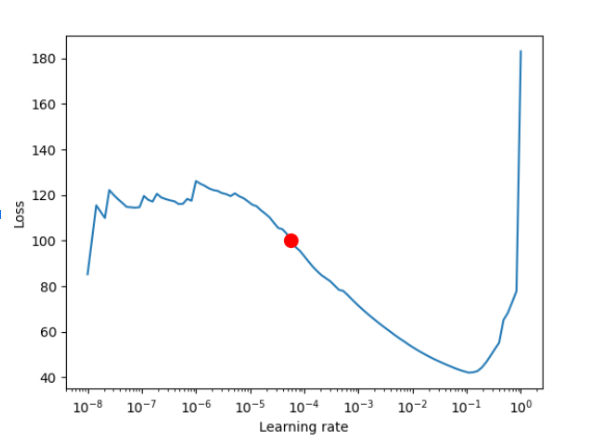
\includegraphics[width=\linewidth]{learningRate30.png}
    \caption{Learning rate vs. loss for 30 epochs}
    \label{fig:lr_30}
  \end{subfigure}
  \hfill
  \begin{subfigure}{0.48\textwidth}
    \centering
    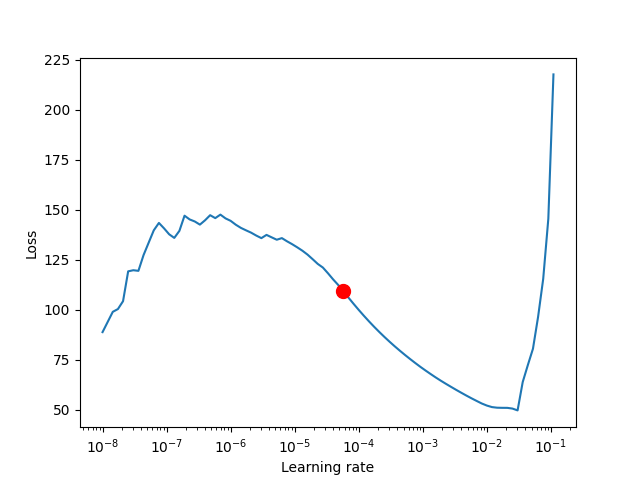
\includegraphics[width=\linewidth]{learningRate150.png}
    \caption{Learning rate vs. loss for 150 epochs}
    \label{fig:lr_150}
  \end{subfigure}
  \caption{One Cycle Learning Rate scheduler performance showing the relationship between learning rate and loss. The steep slope in the range of $10^{-3}$ to $10^{-5}$ indicates the optimal learning rate range for our model.}
  \label{fig:lr_loss}
  \end{figure}
  

After graphing the loss versus the learning rate, we saw that the range of $10^{-3}$ to $10^{-5}$ had the steepest slope and was a good range for our global minima and maxima.

\subsection{Architectures}

While the base model of a TDS-Conv Network has proven to be effective with sound wave recognition \citet{hannun}, we attempted to use different architectures in order to bring the CER down. While exploring other architectures, a main concern was how the architecture uses temporal data to relate different features in the data. 

The base model is a Convolutional Neural Network utilizing CTC loss. CNNs are designed to capture spatial features from data. They apply convolutional filters to input data, which makes them particularly effective at detecting local patterns like edges in images or short-term features in waveforms. This makes CNNs well-suited for identifying localized patterns in sound data, but can struggle with capturing long-term dependencies.

A second type of model is a Long Short-Term Memory network, a type of recurrent neural networks that are optimized to handle sequential data. Its architecture allows it to have memory cells that learn what information to store and what to filter out. This allows LSTMs to process temporal data with an ability to look back and store only crucial features of the data. 

The first architecture we attempted was replacing the convolutional encoder with an LSTM encoder. An LSTM by itself did not significantly improve the base model, improving the CER by only 0.24\%. However, this small difference suggested that a more complex LSTM architecture could yield promising results.

One improvement we made was implementing a dual-encoder model adding an LSTM after the TDS-Conv. By chaining these encoders, we decreased our CER by 4\%. The intuition behind this approach is that while the CNN captures spatial features within a window, the LSTM identifies temporal relationships across sequences, resulting in a model that can effectively capture both spatial and temporal dependencies.

We further enhanced the LSTM by integrating attention head mechanisms \citet{zhao}. Attention mechanisms allow models to focus on different parts of the input data independently and weigh their importance when making predictions. By implementing multi-head attention, the LSTM could independently identify distinct features in the data and combine them in a softmax classifier. While attention isn’t integrated directly into a base LSTM model, this experiment introduced us to transformer architectures, which natively implement attention mechanisms.

Transformers have gained popularity for their effectiveness in handling long-range dependencies. Unlike CNNs, which focus on local patterns, and LSTMs, which process data sequentially, transformers use self-attention to weigh the importance of different parts of the input sequence simultaneously. This parallelization makes them more efficient at capturing both short-term and long-term relationships in data. Previous research in automatic speech recognition \cite{synnaeve} found that transformers consistently achieve the lowest error rates, making them an attractive option for our model.

Inspired by these findings, we implemented a transformer model with 8 attention heads, 4 layers, and a size 384 dimension. As with LSTMs, using this model by itself did not perform well, but when combined with a TDS-Conv encoder as part of a dual-encoder model, performed just as well, or exceeded the performance of an TDS-Conv + LSTM model. For high epoch runs, we did initially run into loss explosion, leading to several failed and time consuming runs. We solved this by applying LayerNorms between each transformer layer and between the two encoders.

Our exploration of these architectures highlights the balance between spatial and temporal feature extraction, and the trade-offs between model complexity and performance. By combining the strengths of CNNs, LSTMs, and transformers, we continue to refine our approach to lowering CER and improving sound wave recognition.


\section{Results}

\begin{table}
  \caption{CER Performance comparison of different model configurations}
  \label{tab:model_performance}
  \centering
  \begin{tabular}{lp{2.8cm}ccc}
  \toprule
  \textbf{Model} & \textbf{Tunings} & \textbf{30 Epochs} & \textbf{150 Epochs} & \textbf{150 Epochs} \\
  & & \textbf{Val/Test CER} & \textbf{Val/Test CER} & \textbf{6gram LM} \\
  \midrule
  CNN & Base & 27.603/28.052 & 19.207/21.872 & 14.732/14.718 \\
  CNN & Time Warping & 25.188/22.757 & - & - \\
  CNN & One Cycle LR & 23.416/24.724 & - & - \\
  CNN & AdamW+OneCycle & 23.128/25.070 & - & - \\
  LSTM & AdamW+OneCycle & 24.767/25.243 & - & - \\
  CNN+LSTM & AdamW+OneCycle & 19.782/21.180 & - & - \\
  CNN+LSTM & Prev+Log Mel & 19.140/20.726 & - & - \\
  CNN+LSTM & AdamW+One+Mel & 16.438/19.294 & 13.646/16.522 & 10.766/12.018\\
  Transformer & Prev & 57.066/60.957 & - & - \\
  CNN+Transformer & Prev & 17.678/19.121 & - & - \\
  CNN+Transformer & Prev & 16.902/19.099 & Loss Explosion & - \\
  CNN+Transformer & Prev+LayerNorm & - & 13.602/15.808 & 9.238/10.957 \\
  \bottomrule
  \end{tabular}
  \end{table}
  
  
  \sloppy
  Our experimental results demonstrate significant improvements over the baseline model through a series of optimizations in data augmentation, architecture design, and learning rate strategies. Table~\ref{tab:model_performance} presents a comprehensive comparison of model performance across different configurations.

  The baseline CNN model served as our starting point for comparison. Our initial improvements focused on enhancing this architecture through data augmentation and optimization techniques. Time warping proved particularly effective, providing a notable relative improvement in test performance compared to the baseline at 30 epochs. Further optimization through the One Cycle Learning Rate scheduler yielded additional gains, demonstrating that optimization strategies alone can produce substantial improvements without architectural changes.
  
  We next explored alternative model architectures. A standalone LSTM model with AdamW and OneCycle showed modest improvements over the baseline CNN, but the most substantial gains came from our hybrid CNN+LSTM approach. This architecture demonstrated the complementary nature of these models in capturing both spatial and temporal features of sEMG signals.
  
  The addition of a Log Mel Spectrogram further enhanced the CNN+LSTM model's performance. Our best 30-epoch model emerged when using a standard Mel Spectrogram with frequency adjustments in the CNN+LSTM architecture, achieving a 16.44\%/19.29\% CER—representing a 40.4\% relative improvement in validation and 31.2\% in test performance compared to the baseline.
  
  A pure Transformer architecture without convolutional components performed poorly, but the CNN+Transformer hybrid with Mel Spectrogram achieved competitive results. When adding frequency adjustments, this model performed comparably to our best CNN+LSTM configuration. Notably, our best 30-epoch models achieved lower error rates than the baseline model trained for 150 epochs (19.21\%/21.87\%), demonstrating the effectiveness of our optimization approach for rapid training.
  
  When extended to 150 epochs, both our CNN+LSTM and CNN+Transformer models showed substantial improvements. The CNN+LSTM with Mel Spectrogram and frequency adjustments reached 13.65\%/16.52\% CER, while the CNN+Transformer with LayerNorm achieved slightly better results at 13.60\%/15.81\%. These represent relative improvements of approximately 29\% in validation and 28\% in test performance compared to the baseline at 150 epochs.
  
  Finally, when incorporating a 6-gram language model with the CNN+Transformer at 150 epochs, we achieved our best overall performance of 9.24\%/10.96\% CER, representing a 37.3\% relative improvement over the baseline model's validation performance and 25.5\% relative improvement in test set performance with the same language model.
  
  These results demonstrate two significant achievements: First, our optimized models at just 30 epochs outperformed the baseline model at 150 epochs, validating our approach for accelerated training on consumer hardware. Second, when trained for the full 150 epochs, our models established new performance benchmarks with substantial relative improvements over the baseline.

\subsection{Limitations}
Our biggest limitation in creating personalized models is that the training, validation, and test set were not big enough. Though we used data augmentation to limit the overfitting and produced acceptable results, the accuracy we present through the CER findings is based on one sample for our validation and one sample for our test data. Without other individuals to compare our models across, the accuracy we found may not generalize well to other individuals.

This extends to how we decide the efficacy of our models. Through training the models to 30 epochs, we chose the most effective models of the CNN + LSTM hybrid model and the transformer model and chose to extend the same training to 150 epochs. Other than changing the hyperparameters for the one cycle learning rate, most other hyperparameters were frozen. Had they been optimized for 150 epochs from the start, we may expect to see greater performance.

In addition, transformations were frozen while changing models. We had initially benchmarked each transformation based off of the pure CNN model and decided to tune the hyperparameters of the existing transformations based on it. However, different models interpret spatial and temporal local data differently. While a Mel spectrogram may have assisted the CNN model as it struggles with finding temporal features, it may have skewed performance on an LSTM or transformer architecture.

\section{Discussion}
Our experimental results can be attributed to three complementary strategies: data augmentation, learning rate scheduling/optimization, and architectural innovations.

The success of the Mel spectrogram transformation in enhancing model performance aligns with established knowledge in audio signal processing. While sEMG signals differ from audio, they share important temporal characteristics that benefit from frequency-domain analysis. Our results suggest that the Mel scale's emphasis on lower frequencies through nonlinear spacing effectively captures the essential muscle activation patterns during typing. This transformation was particularly beneficial because it compressed relatively constant low-frequency components while preserving the higher frequency details associated with the fine motor movements of typing.

The hybrid architectures consistently outperformed single-architecture models, highlighting how different architectures can complement each other. The CNN+LSTM architecture's effectiveness likely stems from the CNN's ability to extract local spatial features combined with the LSTM's capacity to model temporal dependencies. Similarly, the CNN+Transformer approach leverages the CNN's efficiency at detecting local patterns while the transformer's self-attention mechanism captures long-range dependencies across the sequence. This combination seems especially valuable for sEMG signals, which contain both spatial (across different sensors) and temporal (sequence of muscle activations) information.

The dramatic improvement from the One Cycle Learning Rate scheduler demonstrates that learning rate scheduling and optimization strategies can be just as important as model architecture for efficient training. Since the One Cycle scheduler is very similar to a Cosine Annealing scheduler with linear warmup, we attribute much of its success to hyperparameter tuning and the use of momentum in the implementation.

Interestingly, we observed that certain data augmentation techniques produced different effects depending on the underlying architecture. Time warping, for instance, significantly improved CNN performance but showed limited benefits for LSTM and transformer-based models. This suggests that time warping captures temporal variations in a similar fashion to the way LSTMs and transformers do inherently. This example shows the importance matching certain data augmentation strategies to specific architectures rather than applying them universally.

\section{Conclusion and Future Work}

This research demonstrates that effective sEMG to keystroke recognition models can be trained efficiently on consumer hardware through strategic combination of data augmentation, learning rate optimization, and architectural innovations. Our hybrid CNN+LSTM and CNN+Transformer models achieved superior performance compared to the baseline while requiring significantly fewer computational resources and training time. The 30-epoch versions of our models outperformed the baseline trained for 150 epochs, while our fully-trained 150-epoch models established new state-of-the-art performance levels for this task.

These results have important implications for the practical deployment of sEMG-based typing interfaces. The ability to train effective personalized models quickly on consumer hardware removes a significant barrier to adoption, making this technology more accessible for applications where individual calibration is necessary. Our approach enables on-device training with minimal resources, allowing for quick calibration periods after which a user can immediately begin typing with just sEMG signal receptors.

Future work may focus on quick hyperparameter searches based on the data. Fine-tuning the hyperparameters could lead to drastically different and more efficient results, further improving the performance of these compact models. In addition, integrating hardware capable of housing this model in sEMG readers directly may be an interesting practical application of this paper. The development of specialized hardware accelerators optimized for these hybrid architectures could further reduce the resources required for both training and inference.

By demonstrating that high-performance sEMG keystroke recognition can be achieved with limited resources, our work contributes to making advanced human-computer interaction more accessible and practical for everyday use, potentially enabling new applications in assistive technology, mobile computing, and extended reality interfaces.

\bibliographystyle{plainnat}
\bibliography{references}

  

\appendix


\end{document}
